\section{Архитектура и модули системы}

Разработанное программное обеспечение является сложным программным комплексом, состоящим из различных модулей:
\begin{itemize}
    \item модуль построения компактной модели PUF;
    \item модуль симуляции PUF;
    \item модуль контроля доступа;
    \item модуль проверки подлинности.
\end{itemize}

Вышеописанные модули опираются на следующие группы классов, разработанные в рамках дипломного проекта:
\begin{itemize}
    \item Библиотека протокола аутентификации. Написана на языке Python. Содержит методы для проведения основных операций, используемых в проктоколе аутентификации.
    \item Библиотека машинного обучения (для построения модели PUF). Написана на языке программирования Haskell и содержит реализацию алгоритма наивного байесовского классификатора (Naive Bayes Classifier), о котором будет рассказано далее.
    \item Набор классов для работы с PUF. Написана на языке Python. Содержит классы для манипуляции с объектами типа Challenge и Response, которые построены на базе битового массива (bitarray). Реализует реализации алгоритмов генерации, сравнения, сложения и других операций над битовыми массивами, необходимых для обработки сингалов PUF.
    \item Слой взаимодействия с устройствами на языке Python. Является легковесным контрактом, предоставляющим единый интерфейс обращения к подключенным устройствам.
\end{itemize}

Общий принцип взаимодействия компонентов и пример сценария использования программной системы приведен на рисунке~\ref{fig:architecture:flow}. В следующих подразделах более подробно описано назначение и устройство каждого из логических модулей ПС.

\afterpage{
  \begin{landscape}
  \thispagestyle{lscape}
  \begin{figure}[t!]
  \centering
    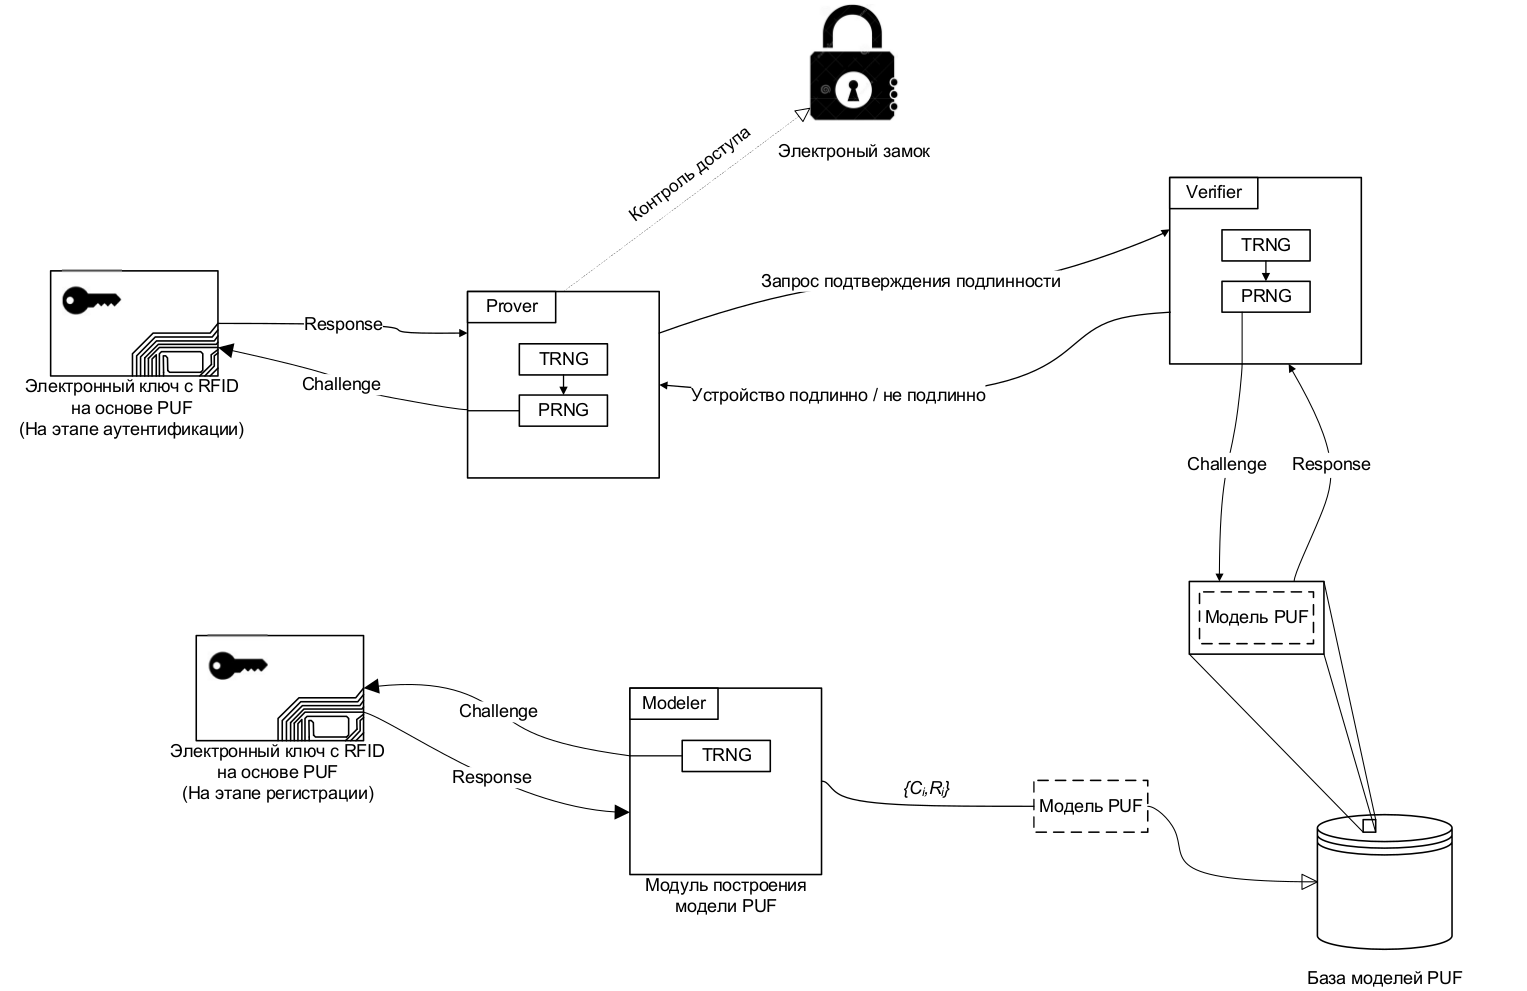
\includegraphics[scale=0.40]{flow.png}
    \caption{ Схема работы программной системы }
    \label{fig:architecture:flow}
  \end{figure}
  \end{landscape}
}


\subsection{Модуль построения компактной модели PUF}
Главная особенность реализуемого протокола аутентификации -- использование компактной модели PUF в качестве эталонного показателя подлинности. Поэтому, закономерно рассмотреть особенности построения этой модели.

Для построения компактной модели ФНФ был выбран наивный байесовский классификатор -- широко используемый метод машинного обучения~\cite{manning_ir}, который при своей относительной простоте реализации, позволяет добиться очень неплохих результатов классификации. На выбор повлияло также то, что задача обучения модели ФНФ сводится к задаче классификации множества входных битовых строк $C$ на выходные классы -- <<0>> и <<1>>.

Наивный баейсовский классификатор – семейство простых вероятностных классфикаторов, которые основываются на теореме Байеса. Классификатор использует решающее правило MAP (maximum a posteriori), которое ставит в соответствие объекту наиболее вероятную для него метку и описывается формулой~\cite{mitchell_ml}:
\begin{equation}
  \label{eq:architecture:bayes}
  y = \underset{c\,\in\,C}{argmax}~P(C) \prod\limits_{i=1}^{n} P(x_i|C)
\end{equation}
\begin{explanation}
где & $ P(C) $ & априорная вероятность принадлежности объекта к классу $C$; \\
    & $ P(x_i|C) $ & правдоподобие принадлежности объекта к классу $C$, исходя из значения аттрибута
$x_i$; \\
    & $ x_i $ & атрибут объекта.
\end{explanation}

При работе с непрерывными аттрибутами используется предположение, что аттрибуты выбираются из независимых непрерывных нормальных распределений. Таким образом, задача обучения классификатора заключается в нахождении параметров распределения -- математического ожидания и дисперсии -- для каждого из аттрибутов, что позволит вычислять $P(x_i|C)$.

Известно, что величины случайных отклонений, связанные с вариацией технологического процесса, подчняются нормальному распределению. Поэтому вполне очевидным является использование байесовского классификатора на основе нормального закона распределения:
\begin{equation}
  \label{eq:architecture:gaussian_bayes}
  P(x_i = \nu|C) = \frac{1}{\sqrt{2 \pi {\sigma}_{ic}^2}} \, exp(-\frac{\nu - \overline{x_{ic}}^2}{2\sigma_{ic}^2})
\end{equation}
\begin{explanation}
где & $x_{ic}$ & среднее значение атрибута, рассчитанное для объектов, принадлежащих
классу $C$; \\
    & $ \sigma_{ic}^2 $ & выборочная дисперсия значания атрибута объектов из класс $C$.
\end{explanation}

Выборочная дисперсия значения атрибута определяется формулой:
\begin{equation}
  \label{eq:architecture:dispersion}
  \sigma_{ic}^2 = \frac{1}{n - 1} \sum\limits_{x \in C} (x_i - \overline{x_{ic}}^2)
\end{equation}

В нашем случае, когда классифицируемыми объектами являются битовые массивы, удобно представить их виде векторов $s$ значених их битов: $s_i \in \{0, 1\}$. Тогда каждый бит массива будет являться атрибутом классифицируемого объекта. В дополнение к этому, благодаря ограниченному набору значений атрибутов ($\{0, 1\}$), вычисления можно значительно оптимизировать.

Модуль построения компактной модели PUF реализован на языке Haskell. На рисунке TODO представлена схема алгоритма классификатора. Листинги \ref{lst:architecture:naive_bayes_hs} и \ref{lst:architecture:statistics_hs} содержит фрагменты кода программного модуля, непосредственно относящиеся к решению задачи классификации. Модуль классификатора поддерживает работу в параллельном режиме на многопроцессорных устройствах, что значительно сокращает время обучения модели.


\lstinputlisting[
    style=commonstyle,
    caption={Наивный байесовский классификатор},
    label=lst:architecture:naive_bayes_hs
]{src/NaiveBayes.hs}

\lstinputlisting[
    style=commonstyle,
    caption={Статистические функции, используемые в классификаторе},
    label=lst:architecture:statistics_hs
]{src/Statistics.hs}

\begin{figure}[!h]
    \centering
    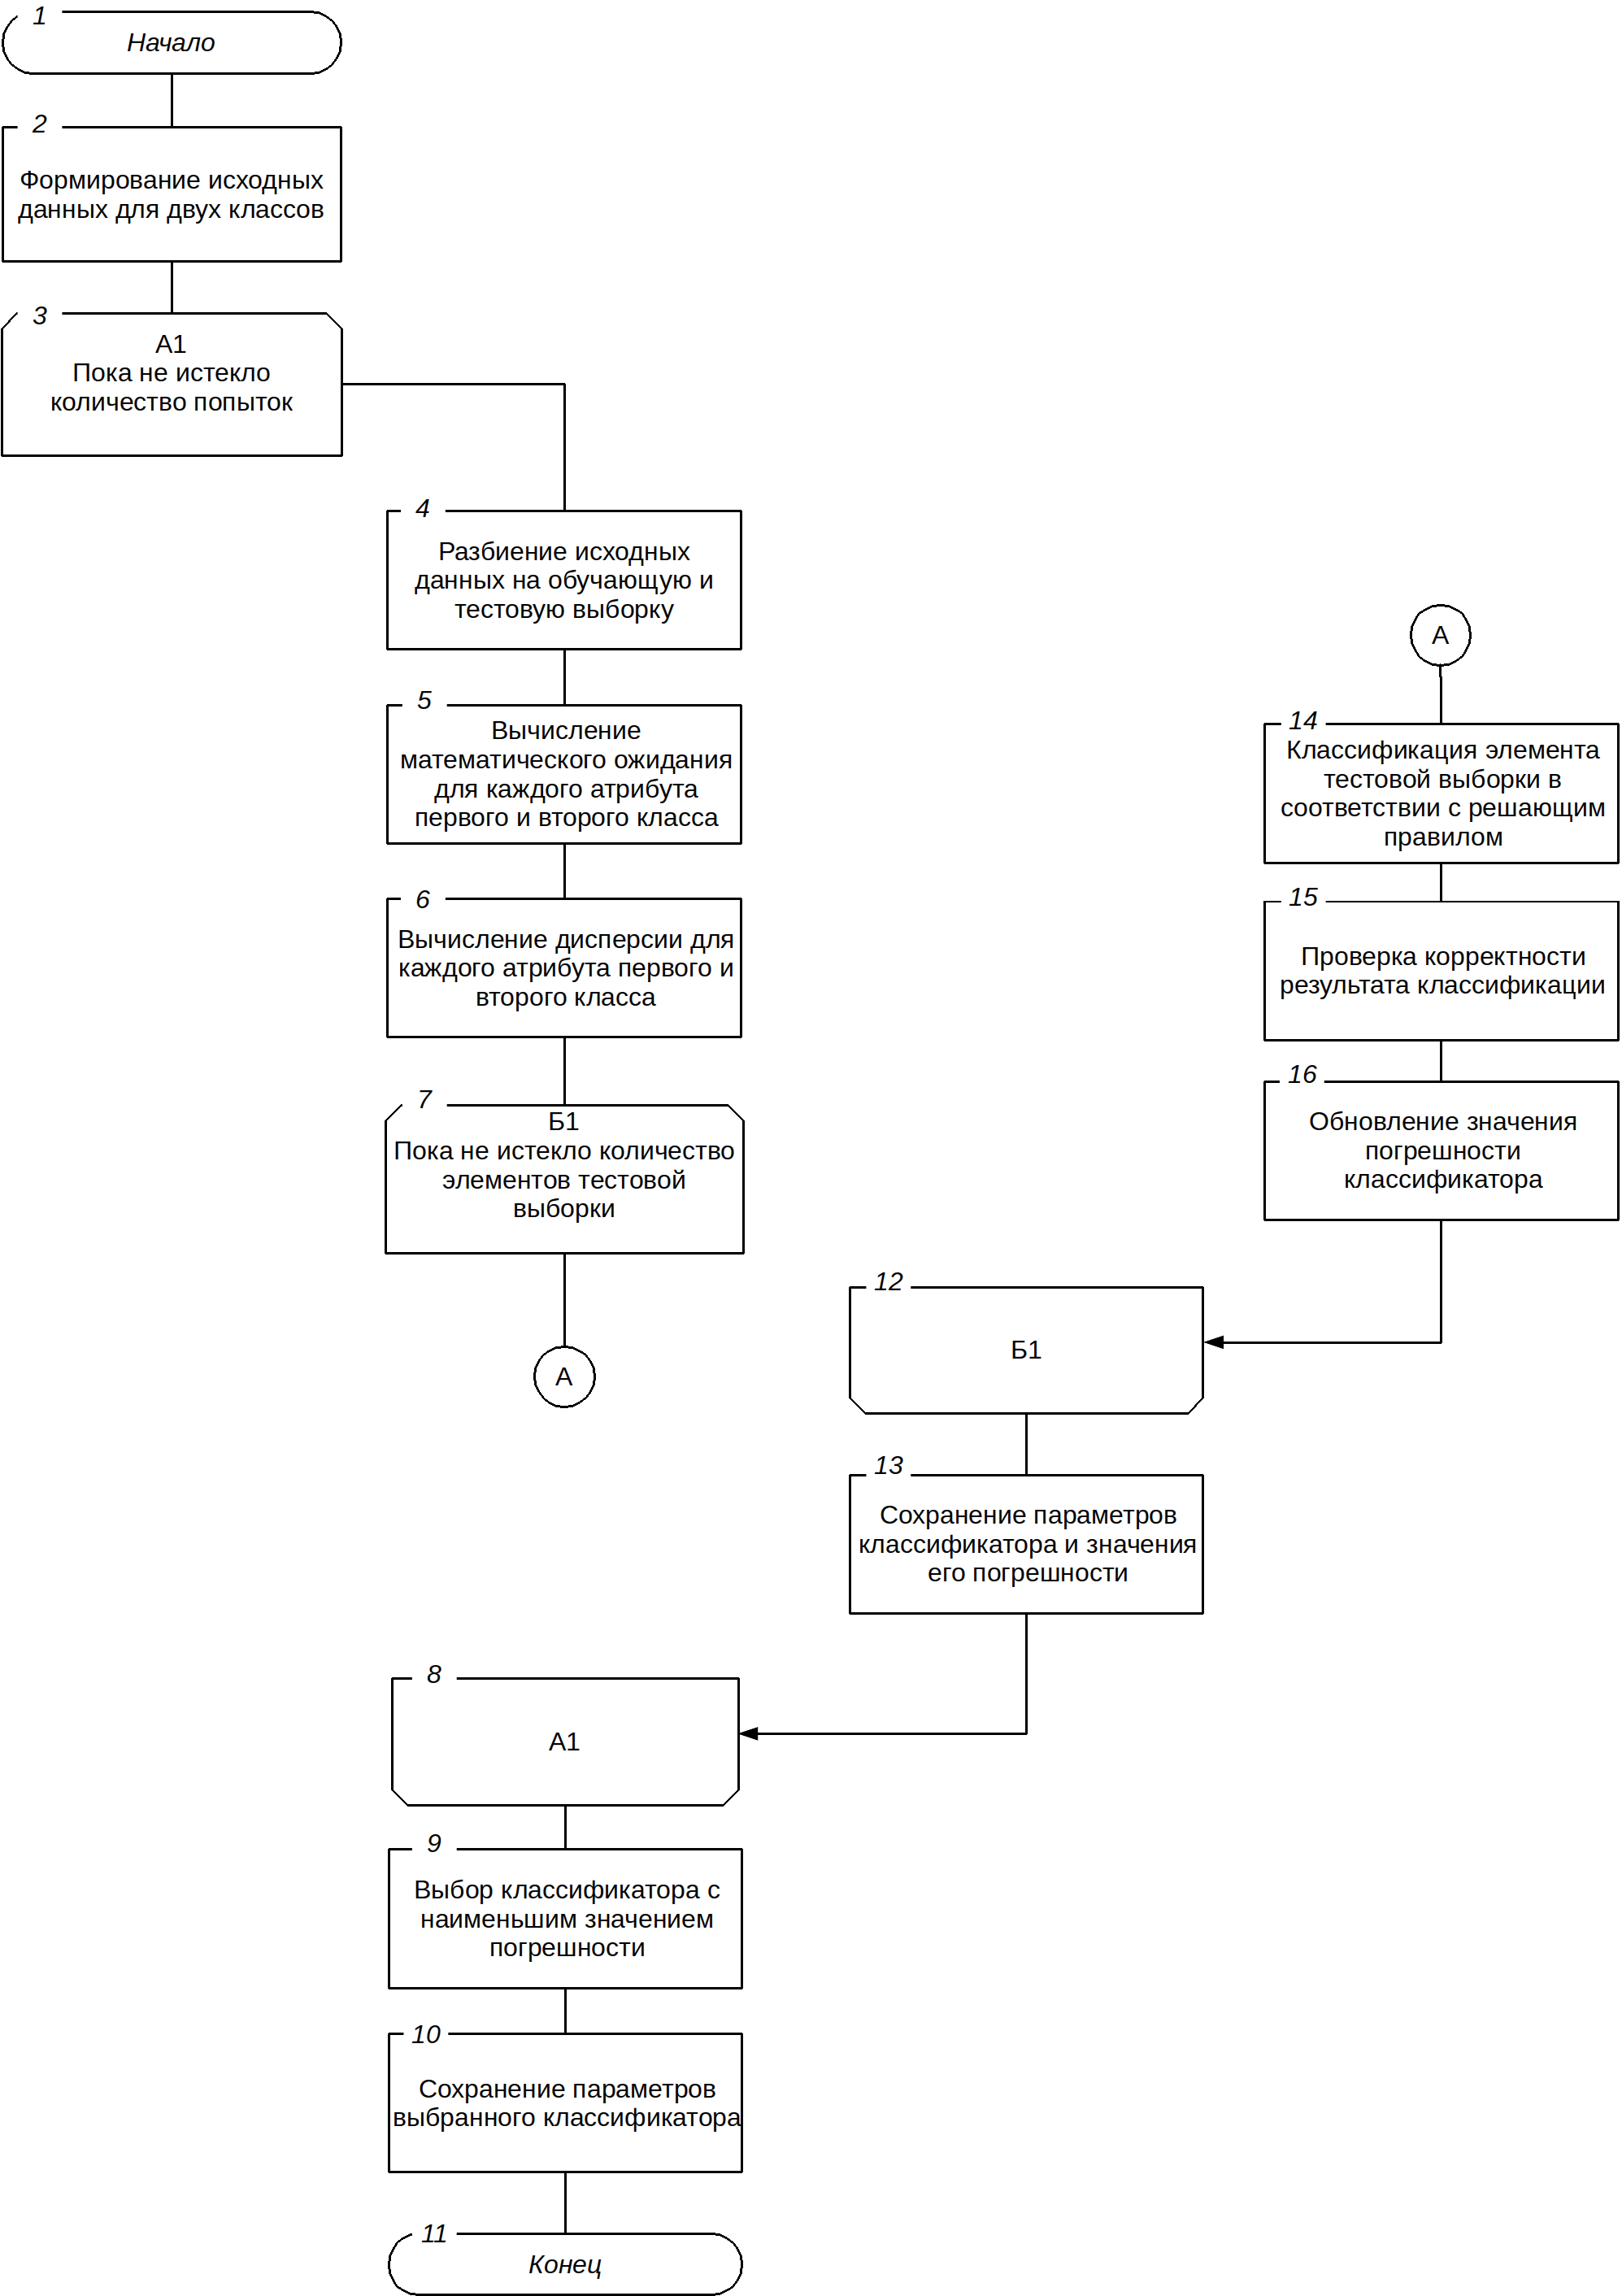
\includegraphics[width=0.95\textwidth]{bayes.png}
    \caption{Схема алгоритма обучения модели методом наивного байесовского классификатора}
    \label{fig:architecture:bayes}
\end{figure}

\subsection{Модуль симуляции PUF}
В целях упрощения разработки, тестирования и демонстрации функциональности ПС было принято решение использовать программную симуляцию физически неклонируемой функции вместо аппаратной реализации. Более того, симуляция PUF может применяться также и конечным пользователем, к примеру, для моделирования PUF со статистическими параметрами, приближенными к таковым у реальной PUF и определения оптимальных параметров функционирования протокола. Таким образом, симуляция PUF из удобного инструмента на этапе разработки переросла в одну из функций программного средства.

Принцип генераций случайных величин, которые будут использованы в качестве физических параметров виртуальной PUF, основан на том факте, что естественные отклонения физических параметров транзисторов (длина, ширина, толщина оксидной плёнки) от заданных значений на этапе их изготовления моделируются распределением, близким к нормальному, так как являются следствиями недетерминированных физических процессов~\cite{gauss_wiki,process_variation}.

\begin{figure}[!h]
    \centering
    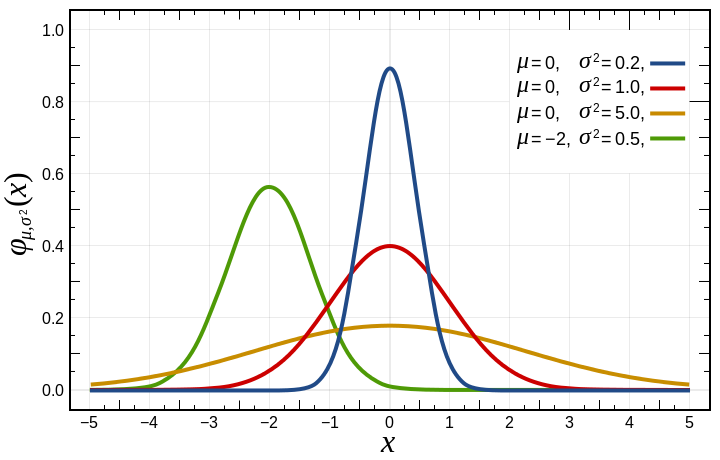
\includegraphics[width=0.85\textwidth]{gauss.png}
    \caption{График функции плотности вероятности для нормального распределения}
    \label{fig:architecture:normal_pd}
\end{figure}

При симуляции физически неклонируемой функции важно учитывать некоторые статистические характеристики, обусловленные нормальным законом распределения значений величин отклонений физических параметров. В частности, из данного факта следует следующее:
\begin{itemize}
  \item Вероятность получения на выходе единицы равна вероятности получения на выходе нуля для всего множества векторов входных сигналов, т.е. $P(r = 0) = P(r = 1) = 0,5 $. Следовательно, в идеальном случае ровно половина возможных векторов входных сигналов соответствует единице на выходе, и ровно половина -- нулю.
  \item Ответы на похожие запросы имеют большую вероятность совпадения. Под похожими понимаются запросы с минимальным расстояниями между ними, рассчитанным по формуле Хэмминга. Иными словами, вероятность того, что ответы $r_0$ и $r_1$ на запросы $C_0$ и $C_1$ будут иметь разные значения, является монотонно возрастающей функцией от расстояния Хэмминга между запросами, т.е. $P(r_0 \neq r_1) = f(HD(C_0, C_1))$. На рисунке ФФФ показана данная зависимость на основании экспериментальных данных.
\end{itemize}

\begin{figure}[!h]
    \centering
    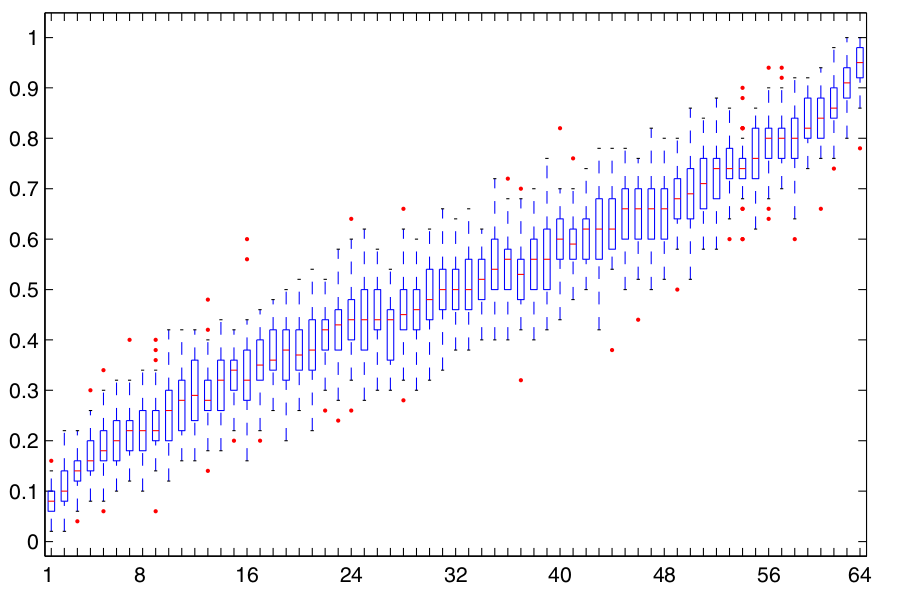
\includegraphics[width=0.75\textwidth]{avalanche.png}
    \caption{График влияния различия входных сигналов на вероятность различия выходных}
    \label{fig:architecture:avalanche}
\end{figure}

При идеальном распределении величин отклонений по нормальному закону выполняется строгий лавинный критерий~\cite{rfid0_puf}, который гласит, что при изменении одного бита аргумента функции выходной бит меняет значение на противоположное с вероятностью 1/2.

Не стоит также забывать, что случайная природа ФНФ не ограничивается лишь вариациями процесса изготовления устройства. Свою случайную компоненту также вносит так называемый <<шум>> -- физические условия окружающей среды, влияющие на параметры полупроводникового устройства. Наиболее остро ощущается влияние высоких температур, при которых функционирует устройство.

Таким образом, для симуляции PUF необходимо учитывать задержки распространения сигналов, привнесенные на этапе производства, а также влияния внешней среды, корректирующие значения этих параметров во время функционирования устройства. Код, используемый для симуляции PUF в программном средстве, учитывает оба эти компонента.

\lstinputlisting[
    style=commonstyle,
    caption={Функиции, используемые для симуляции ФНФ},
    label=lst:architecture:puf_sim
]{src/ropuf.py}


\subsection{Слой взаимодействия с устройствами}
Данная часть программного средства представляет собой абстракцию над любыми типами устройств с PUF (как аппаратными, так и программно симулированными) и предоставляет единый интерфейс взаимодействия с ними. Таким образом, благодаря этому слою, все части программного средства могут единообразно обращаться к любому подключённому устройству с целью регистрации или аутентификации вне зависимости от реализации этого устройства. Для эффективного взаимодействия в рамках этих целей достаточно лишь иметь доступ к собственно функции PUF для обмена сигналами и к некоторым её свойствам, в частности -- ожидаемой длине входного сигнала. С точки зрения программного кода этот слой реализован в виде абстрактного класса device.Device, исходный код которого представлен в листинге \ref{lst:architecture:device}.

\lstinputlisting[
    style=commonstyle,
    caption={Слой взаимодействия с устройствами, класс Device},
    label=lst:architecture:device
]{src/device.py}

В текущей поставке программной системы реализован класс SoftwareArbiter, который представляет собой обертку над программно-симулированным устройством с PUF типа арбитр. Объект класса SoftwareArbiter инициализируется заранее рассчитанными значениями задержек на узлах PUF. Для использования SoftwareArbiter, как и любого другого класса, реализующего методы Device, достаточно вызвать метод объекта SoftwareArbiter.f с битовым массивом значений управляющих сигналов в качестве аргумента. Применительно к PUF типа арбитр функция f рассчитывает выходной бит по следующей формуле:

\begin{equation}
  \label{eq:architecture:arbiter}
  \sum_{j=1}^{N}(-1)^{\rho_j}\delta_j + \delta_{N+1}\mathop{\lessgtr}_{r=1}^{r=0} 0\text{\,,}
\end{equation}
\begin{explanation}
где & $ \rho_j $ & количество единичных битов входного сигнала; \\
    & $ N $ & количество звеньев в цепи; \\
    & $ \delta_j $ & значение задержки на каждом звене. \\
\end{explanation}



\subsection{Библиотека протокола аутентификации}
Реализация протокола аутентификации, используемая в разработанном ПО, является частным случаем т.н. протоколов аутентификации на основе поиска подстроки (substring matching-based authentication protocol). Данный тип протоколов представил в 2012 году M. Majzoobi под названием \emph{Slender  PUF  protocol}~\cite{slender_puf}.

Протокол предназначен для использования со стойкими физически неклонируемыми функциями (Strong PUFs), является очень легковесным и отлично подходит для реализации в устройствах и системах с ограниченными вычислительными ресурсами. В отличие от уже устоявшейся парадигмы, данный протокол не подразумевает раскрытие полной последовательности выходных сигналов, даже в зашифрованном или трансформированном каким-либо другим способом виде. Вместо этого, из последовательности выделяются случайные части и отсылаются как доказательство подлинности. Для аутентификации устройства проверяющая сторона использует заранее сгенерированные шаблоны выходной последовательности (response patterns).

При корректной реализации протокол может обеспечить превосходную устойчивость против любых известных атак, использующих построение модели PUF-устройства с помошью методов машинного обучения. В дополнение к этому, в протокол сразу заложена коррекция ошибок, которые могут возникнуть при получении выходной строки по уже рассмотренным причинам. Благодаря этому, не требуется реализация сторонних алгоритмов коррекции ошибок, отнимающих драгоценные ресурсы, как не требуется и реализация хэш-функций, нечетких экстракторов (fuzzy extractors), предложенных в ранее известных протоколах аутентификации на основе ФНФ.

В основе протокола лежит построение компактной модели PUF методом машинного обучения. При этом оговаривается, что обучение модели должно быть доступно только на этапе регистрации, после чего возможность извлечения полных выходных последовательностей должна быть заблокировано физическим путем.

Библиотека протокола аутентификации представляет собой небольшой набор классов и функций, реализующих протокол аутентификации PUF на основе поиска подстроки. Сама схема протокола аутентификации продемонстрирована на рисунке \ref{fig:architecture:protocol}.

% \afterpage{
\begin{figure}[!h]
    \centering
    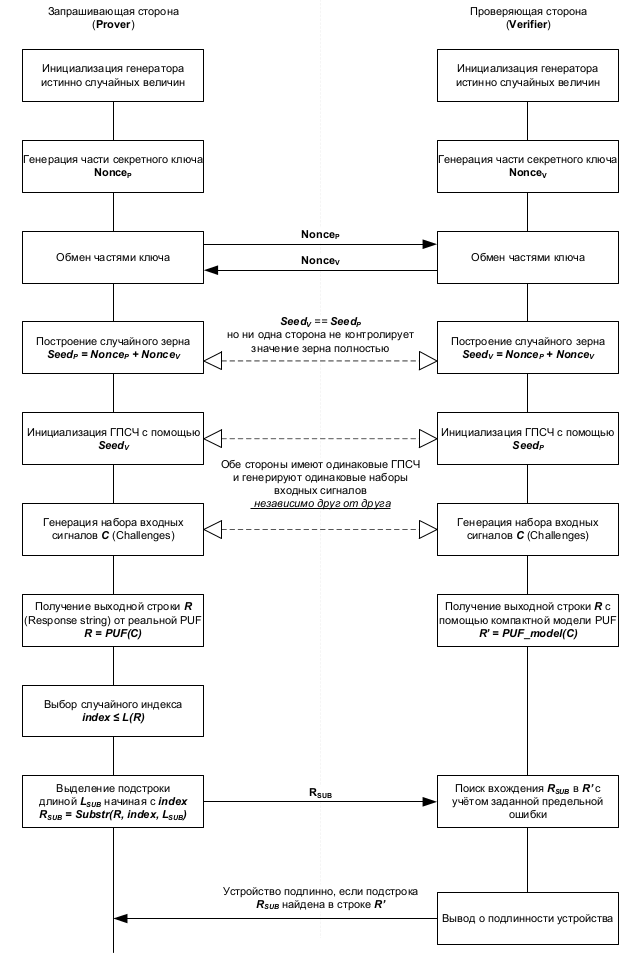
\includegraphics[width=0.93\textwidth]{protocol.png}
    \caption{Схема протокола аутентификации}
    \label{fig:architecture:protocol}
\end{figure}
% }

\clearpage
Набор функций, реализованных в библиотеке, напрямую определяется требованиями протокола. Библиотека предоставляет следующий функционал, используемый как клиентской, так и серверной частью:
\begin{itemize}
  \item Класс-обёртка TRNG для генерации истинно случайных значений с использованием системного генератора случайных чисел. Например в ОС Linux таковым является специальное устройство \emph{/dev/urandom}, предоставляющее интерфейс к пулу случайной информации, сгенерированной драйверами устройств путём сбора метрик шумовых процессов, протекающих при их работе. Применительно к протоколу TRNG используется для получения случайного зерна для PRNG и случайного индекса выходной подпоследовательности в режиме аутентификации и генерации запросов \emph{Challenge} для обучения модели в режиме регистрации.
  \item Класс-обёртка PRNG для генерации псевдослучайных значений. Использует реализацию алгоритма вихря Мерсенна из стандартной библиотеки языка Python. Требует инициализации с помощью зерна. PRNG используется для генерации запросов \emph{Challenge} в режиме аутентификации.
  \item Абстрактный класс Party для обозначения участников взаимодействия по протоколу. Предоставляет реализующим его классам функционал, общий для всех участников: методы идентификации в системе, методы обмена частями случайного зерна, методы генерации псевдослучайных последовательностей входных запросов.
  \item Класс Verifier, реализующий абстрактный класс Party. Представляет сущность сервера проверки подлинности и содержит методы для этапов протокола, специфичных для проверяющей стороны.
  \item Класс Prover, реализующий абстрактный класс Party. Представляет сущность клиентского приложения, представляющего устройство и содержит методы для этапов протокола, специфичных для стороны, запрашивающей проверку.
  \item Класс Configuration, представляющий собой набор конфигурационных параметров протокола и поддерживает инициализацию с помощью файла настроек или системных переменных окружения в дополнение к инициализации с помощью стандартных параметров конструктора.
\end{itemize}

Класс Configuration разобран чуть подробнее, так как от правильного его использования зависит применение параметров работы протокола, влияющих главным образом, на процент ложных срабатываний или наоборот, ложных отказов.
\clearpage
\lstinputlisting[
    style=commonstyle,
    firstline=5,
    caption={Класс Configuration},
    label=lst:architecture:configuration
]{src/configuration.py}

В таблице \ref{table:architecture:cfg_items} приведены краткие описания доступных параметров:

\begin{table}[ht]
  \caption{Параметры протокола аутентификации}
  \label{table:architecture:cfg_items}
  \begin{tabular}{| >{\raggedright}m{0.45\textwidth}
                  | >{\raggedright\arraybackslash}m{0.5\textwidth}|}
   \hline
   Параметр & Описание
   \\ \hline
   \textit{NONCE\_SIZE} & Длина (в битах) половины случайного зерна (результирующее зерно будет иметь длину \textit{2xNONCE\_SIZE}), используемого для инициализации ГПСЧ
   \\ \hline
   \textit{SUBSTR\_LEN} & Длина (в битах) извлекаемой из ответа реального устройства подстроки
   \\ \hline
   \textit{THRESHOLD} & Максимальное значение расстояния Хэмминга между строками, при котором они всё еще считаются схожими
   \\ \hline
   \textit{RSP\_LEN} & Фиксированная длина (в битах) ответа устройства (используется только для тестирования!)
   \\ \hline
  \end{tabular}
\end{table}

В следующих подразделах будут рассмотрены две стороны, взаимодействующие в рамках протокола.

\subsection{Модуль контроля доступа (клиентская часть)}
Так как протокол аутентификации по сути является набором правил, регулирующих обмен информацией нескольких сторон (в данном случае двух), логично описать правила поведения каждой из сторон по отдельности. В реализуемом протоколе участвуют \emph{клиент} -- сторона, имеющая доступ к устройству и <<представляющая его интересы>> в процессе аутентификации и \emph{сервер} -- сторона, обладающая подтверждение подлинности устройства.

В данной упрощённой реализации клиент также контролирует доступ к ресурсу, запрашиваемому устройством. Простейший пример -- электронный ключ в виде устройства с PUF запрашивает доступ к некоторому ресурсу, защищённому электронным замком. Электронный замок ничего не знает о подлинности устройства, в свою очередь устройство не может в одиночку доказать свою подлинность, т.к. по умолчанию не является доверенным. Здесь устройство пользуется <<услугой>> клиента (Prover), который является посредником между устройством, доказывающим свою подлинность, и доверенным сервером, обладающим релевантной информацией насчёт неё. Посредник также контролирует электронный замок, т.е. контролирует, какие устройства могут иметь к секретному ресурсу по результатам процесса аутентификации. Совмещение ролей посредника и барьера, конечно же, не является обязательным и сделано для упрощения архитектуры программного средства и эти роли могут быть без особых проблем разделены для более тонкого контроля над всей инфраструктурой.

По правилам протокола аутентификации клиентский модуль выполняет следующие функции:
\begin{itemize}
  \item генерировать истинно случайные и псевдослучайные данные для использования в алгоритмах протокола;
  \item взаимодействовать с устройством, посылая наборы входных сигналов и считывая результаты на выходе;
  \item создавать компактную модель уPUF на этапе регистрации;
  \item взаимодействовать с сервером, обмениваясь с ним секретной информацией -- с помощью библиотеки requests и грамотного использования защищенных соединений  и клиентских сессий.
\end{itemize}

С добавлением роли барьера примешиваются дополнительно функции надёжного хранения ссылки на секретный ресурс и предоставления устройству ссылки на секретный ресурс  в случае успешной аутентификации.

Как можно увидеть, модуль клиентской стороны использует множество ранее описанных классов и функций, не описывая своих классов или структур данных. Основной задачей клиентского модуля является реализация алгоритма проведения операций регистрации и атуентификации с использованием уже созданных инструментов. В таблице~\ref{table:architecture:client_funcs} описано, как реализованы эти инструменты, на основе которых построен алгоритм, являющийся главной логикой клиентского модуля.

\begin{table}[ht]
  \caption{Функции клиентского модуля и их реализации}
  \label{table:architecture:client_funcs}
  \begin{tabular}{| >{\raggedright}m{0.45\textwidth}
                  | >{\raggedright\arraybackslash}m{0.5\textwidth}|}
   \hline
   Функция & С помощью чего реализована
   \\ \hline
   Генерация истинно случайных чисел & Класс TRNG модуля протокола аутентификации
   \\ \hline
   Генерация псевдослучайных чисел & Класс PRNG модуля протокола аутентификации
   \\ \hline
   Обмен битовыми строками входных и выходных сигналов с утройствами & Класс Device и его производные классы в слое взаимодействия с устройствами
   \\ \hline
   Создание компактной модели PUF & Класс-обёртка над модулем построения модели (для обеспечения интероперабельности языков Python и Haskell)
   \\ \hline
   Контроль доступа у секретным ресурсам & Внутренние функции модуля или опциональный внешний интерфейс.
   \\ \hline
  \end{tabular}
\end{table}

\subsection{Модуль проверки подлинности (серверная часть)}
В описанном выше протоколе \emph{сервер} является сущностью, располагающей информацией о подлинности зарегистрированных устройств. Эта информация представлена в виде компактных моделей PUF, созданных на этапе их регистрации.

Функционал сервера во многом повторяет таковой у клиента, именно поэтому было принято решение вынести общие функции в абстрактный класс Prover. Сервер использует свою реализацию этого класса -- Verifier.

На основании вышесказанного, серверный модуль проверки подлинности выполняет следующие функции:
\begin{itemize}
  \item генерировать истинно случайные и псевдослучайные данные для использования в алгоритмах протокола;
  \item взаимодействовать с моделью устройства, посылая наборы входных сигналов и считывая результаты на выходе;
  \item иметь доступ к хранилищу моделей PUF;
  \item использовать алгоритм нечеткого поиска строки для сравнения данных, полученных от реального устройства с данными, полученными от компактной модели;
  \item работать в режиме сервера, т.е. принимать и обрабатывать входящие запросы, все время находясь в ожидании новых запросов;
\end{itemize}


\lstinputlisting[
    style=commonstyle,
    firstline=18,
    caption={Метод нечеткого поиска подстроки с заданным порогом},
    label=lst:architecture:fuzzysearch
]{src/fulllisting/puf.py}

\begin{table}[ht]
  \caption{Функции серверного модуля и их реализации}
  \label{table:architecture:client_funcs}
  \begin{tabular}{| >{\raggedright}m{0.45\textwidth}
                  | >{\raggedright\arraybackslash}m{0.5\textwidth}|}
   \hline
   Функция & С помощью чего реализована
   \\ \hline
   Работа в качестве HTTP-сервера по защищенному протоколу & Веб-фреймворка Flask и его поддержка безопасных соединений и клиентских сессий.
   \\ \hline
   Генерация истинно случайных чисел & Класс TRNG модуля протокола аутентификации
   \\ \hline
   Генерация псевдослучайных чисел & Класс PRNG модуля протокола аутентификации
   \\ \hline
   Обмен битовыми строками входных и выходных сигналов с моделью PUF & Класс Model
   \\ \hline
   Работа с хранищилем моделей PUF & Класс Database и его реализации для работы с файловой системой, Redis или MongoDB
   \\ \hline
   Нечеткий поиск подстроки & Класс Response модуля PUF и его реализации нечеткого поиска
   \\ \hline
  \end{tabular}
\end{table}


Сервер проверки подлинности должен иметь возможность обмена данными с моделью образом, похожим на способ взаимодействия с устройствами для модуля контроля доступа. Для данной цели создан класс Model, который предоставляет такой же интерфейс к модели PUF, какой предоставляет слой взаимодействия с устройствами для реальных PUF. Метод \emph{f} класса Model принимает масиив битов класса Challenge и возвращает бит ответа -- объект класса Response.

Для взаимодействия с хранилищем моделей модуль проверки подлинности предоставляет простой класс Database, по умолчанию реализующий хранение моделей в виде файлов на файловой системе. В то время как такой подход может быть полезен при тестировании приложения, для реального использования стоит также рассмотреть другие варианты:
\begin{itemize}
  \item NoSQL база данных. Так как модели PUF являются независимыми наборами векторов, использование классической реляционной базы данных в данном случае нерационально, ведь модели не имеют множества атрибутов, как не имеют и связей и отношений с другими сущностями в БД. В рамках этого варианта программное средство поддерживает работу с нереляционной СУБД MongoDB.
  \item Кэш (неперсистентное хранилище). В зависимости от требований информационной системы, в которой планируется использование данного ПС, является вероятным сценарий того, что модели PUF не должны храниться в базе слишком долго, или даже могут являться одноразовыми. В данном случае можно использовать систему хранения временных данных в памяти (memcached, Redis). Более того, так как в системе принято условие <<одно устройство -- одна модель>>, можно обойтись простейшим хранилищем типа <<ключ-значение>>(\emph{key-value store}). Для этого варианта реализован класс для работы с хранилищем Redis.
\end{itemize}
